\usetikzlibrary{positioning}
\usetikzlibrary{decorations}

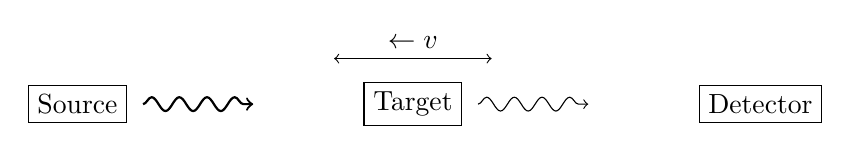
\begin{tikzpicture}
    \node[draw] (source) at (0, 0) {Source};
    \node[draw] (target) [right=3cm of source] {Target};
    \node[draw] (detector) [right=3cm of target] {Detector};

    \draw[->] (target.north) ++(0, 0.3) node[above] {$\leftarrow v$} -- ++(1, 0);
    \draw[->] (target.north) ++(0, 0.3) -- ++(-1, 0);

    \draw[thick, ->, decorate, decoration=snake] (source.east) ++(0.2, 0) -- ++(1.4, 0);
    \draw[->, decorate, decoration=snake] (target.east) ++(0.2, 0) -- ++(1.4, 0);
\end{tikzpicture}
